% !TEX program = xelatex
\documentclass[11pt,aspectratio=43]{beamer}
% !TEX program = xelatex
\usepackage[UTF8,fontset=fandol]{ctex}
\usepackage{amsmath,amssymb,mathtools,booktabs,array,tabularx}
\usepackage{graphicx}
\usepackage{tikz}
\usetikzlibrary{arrows.meta,positioning,calc}
\usetheme{Warsaw}
% lec1.pdf proportions and Warsaw framing, with coordinated semantic block colors.
\definecolor{lecblue}{RGB}{20,40,80}
\definecolor{lecmid}{RGB}{15,30,60}
\definecolor{lecdark}{RGB}{10,20,40}
\definecolor{lecgray}{RGB}{231,232,235}
\definecolor{defhead}{HTML}{D6E2EF}
\definecolor{defbody}{HTML}{EFF3F8}
\definecolor{defink}{HTML}{294C70}
\definecolor{thmhead}{HTML}{D2E4DC}
\definecolor{thmbody}{HTML}{EDF4F0}
\definecolor{thmink}{HTML}{325D52}
\definecolor{remhead}{HTML}{EBE1CF}
\definecolor{rembody}{HTML}{F8F4EC}
\definecolor{remink}{HTML}{766448}
\setbeamercolor{structure}{fg=lecblue}
\setbeamercolor{palette primary}{fg=white,bg=lecblue}
\setbeamercolor{palette secondary}{fg=white,bg=lecmid}
\setbeamercolor{palette tertiary}{fg=white,bg=lecdark}
\setbeamercolor{palette quaternary}{fg=white,bg=lecdark}
\setbeamercolor{frametitle}{fg=white,bg=lecblue}
\setbeamercolor{frametitle right}{fg=white,bg=lecdark}
\setbeamercolor{title}{fg=white,bg=lecblue}
\setbeamercolor{author}{fg=defink}
\setbeamercolor{institute}{fg=black}
\setbeamercolor{block title}{fg=defink,bg=defhead}
\setbeamercolor{block body}{fg=black,bg=defbody}
\setbeamercolor{alerted text}{fg=defink}
\setbeamercolor{author in head/foot}{fg=white,bg=lecmid}
\setbeamercolor{section in head/foot}{fg=white,bg=lecblue}
\setbeamercolor{date in head/foot}{fg=white,bg=defink}
\setbeamercolor{section in toc}{fg=lecblue}
\setbeamertemplate{navigation symbols}{}
\setbeamertemplate{headline}{}
\newcommand{\currentmajor}{Paper Presentation}
\setbeamertemplate{footline}{%
 \leavevmode\hbox{%
 \begin{beamercolorbox}[wd=.42\paperwidth,ht=2.6ex,dp=1.1ex,center]{author in head/foot}%
 \fontsize{6.5}{8}\selectfont\insertshortinstitute
 \end{beamercolorbox}%
 \begin{beamercolorbox}[wd=.27\paperwidth,ht=2.6ex,dp=1.1ex,center]{section in head/foot}%
 \fontsize{6.5}{8}\selectfont\currentmajor
 \end{beamercolorbox}%
 \begin{beamercolorbox}[wd=.31\paperwidth,ht=2.6ex,dp=1.1ex,leftskip=.15cm,rightskip=.15cm]{date in head/foot}%
 \fontsize{6.5}{8}\selectfont\insertshortdate\hfill\insertframenumber/\inserttotalframenumber
 \end{beamercolorbox}}}
\setbeamersize{text margin left=.4cm,text margin right=.4cm}
\setbeamertemplate{section in toc}[ball]
\setbeamertemplate{enumerate items}[ball]
\setbeamertemplate{itemize items}[ball]
\setlength{\parskip}{1pt}
\newcommand{\R}{\mathbb R}
\newcommand{\blue}[1]{{\color{defink}#1}}
\newenvironment{definitionbox}[1]{\begin{block}{#1}}{\end{block}}
\newenvironment{theorembox}[1]{\begingroup
 \setbeamercolor{block title}{fg=thmink,bg=thmhead}
 \setbeamercolor{block body}{fg=black,bg=thmbody}
 \begin{block}{#1}}{\end{block}\endgroup}
\newenvironment{remarkbox}[1]{\begingroup
 \setbeamercolor{block title}{fg=remink,bg=remhead}
 \setbeamercolor{block body}{fg=black,bg=rembody}
 \begin{block}{#1}}{\end{block}\endgroup}
\newcommand{\tight}{\setlength{\abovedisplayskip}{5pt}\setlength{\belowdisplayskip}{5pt}\setlength{\abovedisplayshortskip}{3pt}\setlength{\belowdisplayshortskip}{3pt}}
\newcolumntype{L}[1]{>{\raggedright\arraybackslash}p{#1}}
\tikzset{box/.style={draw=defink!65,fill=defbody,rounded corners=2pt,align=center,font=\footnotesize,inner sep=4pt,minimum height=.8cm},
 arr/.style={-{Latex[length=1.7mm]},thick,lecmid},
 labeltext/.style={fill=white,inner sep=2pt,font=\scriptsize,text=lecmid}}

\usepackage{microtype}
\newcommand{\src}[1]{\par\vspace{2pt}{\fontsize{6.5}{7.5}\selectfont\color{defink}#1\par}}
\newcommand{\major}[1]{\renewcommand{\currentmajor}{#1}}
\newcommand{\tbl}{\renewcommand{\arraystretch}{1.16}\setlength{\tabcolsep}{3pt}}
\hypersetup{colorlinks=true,urlcolor=defink,linkcolor=lecblue,pdfauthor={Tongren Xiao},pdftitle={Design of a Specialized Tokenizer for Mathematical Text}}
\title[Math Tokenization]{\texorpdfstring{Design of a Specialized Tokenizer\\[1ex]for Mathematical Text}{Design of a Specialized Tokenizer for Mathematical Text}}
\author[Tongren Xiao]{\texorpdfstring{Tongren Xiao\\[1ex]\texttt{tongrenxiao7@gmail.com}}{Tongren Xiao}}
\institute{Department of Mathematics, Sun Yat-sen University}
\date[October 10, 2026]{October 10, 2026}
\begin{document}
\footnotesize\tight
\major{Research Presentation}
\begin{frame}[noframenumbering]\titlepage
\note{Cover identity, email, institute and date are retained from the supplied GBFR reference. The research artifacts and literature search were updated on October 13, 2026.}
\end{frame}

\major{Research Question}
\begin{frame}[t]{Can Mathematical Tokenization Improve Model Capability?}
\relax
\begin{definitionbox}{Research question}
Can we train tokenizers specifically for mathematical text that improve both \textbf{intrinsic tokenization} and \textbf{downstream mathematical capability}?
\end{definitionbox}
\vspace{8pt}\par\noindent{\footnotesize\renewcommand{\tbl}{\renewcommand{\arraystretch}{2.3}\setlength{\tabcolsep}{3pt}}\tbl\begin{tabularx}{\linewidth}{@{}L{3.0cm}>{\raggedright\arraybackslash}X@{}}\toprule
Question & What would count as evidence?\\\midrule
RQ1: tokenizer quality & Lossless compression, robustness, speed, etc.\\
RQ2: model capability & Mathematical tasks such as PDE/ODE solving.\\
Current status & Tokenizer experiments completed; downstream evaluation to follow.\\
\bottomrule\end{tabularx}}\par\vspace{2pt}

\note{This page is intentionally limited to the research question and requested short evidence descriptions.}

\end{frame}

\major{Research Question}
\begin{frame}[t]{Study Overview}
\relax
\par\noindent{\footnotesize\renewcommand{\tbl}{\renewcommand{\arraystretch}{2.8}\setlength{\tabcolsep}{5pt}}\tbl\begin{tabularx}{\linewidth}{@{}L{2.4cm}>{\raggedright\arraybackslash}X@{}}\toprule
Component & Summary\\\midrule
Dataset & We constructed and classified a dataset of mathematical formulas from multiple mathematical fields.\\
Models & We proposed two specialized mathematical tokenizers.\\
Baselines & We selected five tokenizers: classical BPE and Unigram methods, and tokenizers used by mature large language models.\\
Results & Our two tokenizers achieve leading performance on core intrinsic metrics and in the overall comparison.\\
\bottomrule\end{tabularx}}\par\vspace{2pt}

\note{Leading performance refers to selected core metrics and the stated aggregate comparison; the experimental tables do not show universal dominance on every individual metric.}

\end{frame}

\major{Baseline}
\begin{frame}[t]{Baseline Tokenizers}
\relax
\par\noindent{\scriptsize\renewcommand{\tbl}{\renewcommand{\arraystretch}{1.8}\setlength{\tabcolsep}{3pt}}\tbl\begin{tabularx}{\linewidth}{@{}L{2.4cm}L{1.5cm}L{1.7cm}>{\raggedright\arraybackslash}X@{}}\toprule
Category & Tokenizer & Actual ID space & Code / tokenizer source\\\midrule
Classical tokenizers & Byte BPE \hyperlink{ref-bpe}{(1)} & 1,024 / 2,048 & \href{https://github.com/huggingface/tokenizers}{huggingface/tokenizers}\\
Classical tokenizers & SP Unigram \hyperlink{ref-sentencepiece}{(2)} & 1,024 / 2,048 & \href{https://github.com/google/sentencepiece}{google/sentencepiece}\\
General-Purpose Tokenizers & Qwen2.5 \hyperlink{ref-qwen}{(3)} & 151,665 & \href{https://huggingface.co/Qwen/Qwen2.5-0.5B/blob/main/tokenizer.json}{Qwen2.5-0.5B/tokenizer.json}\\
General-Purpose Tokenizers & Llama 3 \hyperlink{ref-llama}{(4)} & 128,256 & \href{https://github.com/meta-llama/llama3/blob/a0940f9cf7065d45bb6675660f80d305c041a754/llama/tokenizer.py}{meta-llama/llama3/tokenizer.py}\\
General-Purpose Tokenizers & o200k \hyperlink{ref-tiktoken}{(5)} & 200,019 & \href{https://github.com/openai/tiktoken}{openai/tiktoken}\\
\bottomrule\end{tabularx}}\par\vspace{2pt}
\vspace{6pt}\begin{itemize}
\item Qwen2.5: used by the Qwen2.5 model family.
\item Llama 3: used by the Meta Llama 3 model family.
\item o200k\_base: used by GPT-4o and GPT-4.1.
\end{itemize}

\note{Source links point to the actual public implementation or tokenizer artifact used. Actual ID spaces are taken from the frozen active registry; SP Unigram includes byte fallback IDs.}

\end{frame}

\major{Baseline}
\begin{frame}[t]{SP Unigram: Training and Inference}
\relax
\par\noindent{\scriptsize\renewcommand{\tbl}{\renewcommand{\arraystretch}{1.35}\setlength{\tabcolsep}{3pt}}\tbl\begin{tabularx}{\linewidth}{@{}L{2.1cm}>{\raggedright\arraybackslash}X@{}}\toprule
Training step & Procedure\\\midrule
Preparation & Use raw strings without language-specific word segmentation; represent spaces as a symbol, usually {\fontspec{Apple Symbols}▁}.\\
1. Initialize & Create a large seed vocabulary of characters, frequent substrings and symbols; assign initial piece probabilities.\\
2. EM iterations & E: sum over possible segmentations to obtain expected piece counts. M: re-estimate probabilities from those counts.\\
3. Prune & Remove pieces with low contribution to corpus likelihood; repeat EM and pruning to reach 1,024 or 2,048 IDs.\\
4. Final model & A piece vocabulary and probabilities; an optional byte fallback table.\\
\bottomrule\end{tabularx}}\par\vspace{2pt}
\vspace{2pt}\textbf{Inference}\par Build a segmentation lattice; for \texttt{abc}: $a+b+c$, $ab+c$, $a+bc$, or $abc$.\[P(s)=\prod_i p(s_i),\qquad s^*=\arg\max_{s\in\mathcal S(x)}P(s).\]Viterbi dynamic programming returns the most probable token sequence. \hyperlink{ref-unigram}{(6)} \hyperlink{ref-sentencepiece}{(2)}
\note{Raw training describes the SentencePiece approach. For this experiment identity normalization and whitespace-preserving settings are used. E-step uses forward/backward dynamic programming rather than explicit exponential enumeration. P(s) is one segmentation probability; the training string likelihood is P(x)=sum_s P(s). Official SentencePiece uses a Bayesian/digamma probability update and loss-based pruning, so the next example illustrates basic maximum-likelihood EM rather than byte-for-byte trainer behavior. U+2581 denotes the visible space symbol.}

\end{frame}

\major{Baseline}
\begin{frame}[t]{SP Unigram: A Two-Round EM Example}
\relax
\textbf{Setup:} one training string \texttt{ab}; pieces $a,b,ab$; initially $p(a)=p(b)=p(ab)=1/3$.\par\vspace{3pt}\textbf{E step: segmentation likelihoods and posteriors}\par\par\noindent{\scriptsize\tbl\begin{tabularx}{\linewidth}{@{}L{1cm}L{2.5cm}L{1.5cm}L{1cm}>{\raggedright\arraybackslash}X@{}}\toprule
Round & $(a,b)$ likelihood & $ab$ likelihood & $P(x)$ & Posterior: $(a,b)$ / $ab$\\\midrule
1 & $1/3\times1/3=1/9$ & $1/3=3/9$ & $4/9$ & $1/4=0.25$ / $3/4=0.75$\\
2 & $0.2\times0.2=0.04$ & $0.6$ & $0.64$ & $0.0625$ / $0.9375$\\
\bottomrule\end{tabularx}}\par\vspace{2pt}
\vspace{4pt}\textbf{M step: expected counts and normalized probabilities}\par\par\noindent{\scriptsize\tbl\begin{tabularx}{\linewidth}{@{}L{1cm}L{3.5cm}L{1cm}>{\raggedright\arraybackslash}X@{}}\toprule
Round & $\mathbb E[n_a],\mathbb E[n_b],\mathbb E[n_{ab}]$ & Total & $p(a),p(b),p(ab)$\\\midrule
1 & $0.25,\;0.25,\;0.75$ & $1.25$ & $0.2,\;0.2,\;0.6$\\
2 & $0.0625,\;0.0625,\;0.9375$ & $1.0625$ & $1/17,\;1/17,\;15/17$\newline $\approx0.0588,\;0.0588,\;0.8824$\\
\bottomrule\end{tabularx}}\par\vspace{2pt}
\[P(x)=\sum_{s\in\mathcal S(x)}\prod_i p(s_i),\qquad p(v)=\frac{\mathbb E[n_v]}{\sum_u\mathbb E[n_u]}.\]For this one-string example, $p(ab)\to1$ and $p(a),p(b)\to0$: EM favors the whole piece $ab$. Low-contribution pieces become pruning candidates; required characters remain protected. \hyperlink{ref-unigram}{(6)}
\note{Simplified maximum-likelihood EM example supplied by the user; exact arithmetic was checked with rational numbers. Real SentencePiece uses a Bayesian probability update, estimates pruning loss, and preserves required symbols. The toy example cannot imply universal deletion of individual characters.}

\end{frame}

\major{Related Work}
\begin{frame}[t]{Our Two Routes: Contribution and Prior Art}
\relax
\par\noindent{\scriptsize\tbl\begin{tabularx}{\linewidth}{@{}L{2.2cm}>{\raggedright\arraybackslash}X >{\raggedright\arraybackslash}X@{}}\toprule
Dimension & Math-atom BPE & Boundary AST\\\midrule
Vocabulary & Fit-derived complete-command/Unicode atoms; original BPE. & Exactly the same byte vocabulary and ID budget.\\
Segmentation & Original learned BPE merge order. & Minimum additive token/tree/boundary cost on a legal source graph.\\
Mathematical prior & Lexical units observed in training. & Lexical units plus a restricted source parser.\\
Deployment & Native reversible codec + original Rust BPE. & Fused native trie traversal and dynamic programming.\\
Novelty boundary & A reproducible domain-specific training recipe. & A tested structural trade-off; shortest paths and AST ideas are not new.\\
\bottomrule\end{tabularx}}\par\vspace{2pt}
\begin{remarkbox}{Central comparison}
Holding the dictionary fixed isolates the effect of the structural segmentation rule. Comparing against generic tokenizers instead measures the complete specialized system.
\hyperlink{ref-cmer}{(7)} \hyperlink{ref-pathpiece}{(8)} \hyperlink{ref-mathgpt}{(9)}
\end{remarkbox}

\end{frame}

\major{Dataset}
\begin{frame}[t]{Dataset}
\relax
\par\noindent{\footnotesize\renewcommand{\tbl}{\renewcommand{\arraystretch}{1.8}\setlength{\tabcolsep}{3pt}}\tbl\begin{tabularx}{\linewidth}{@{}L{3.2cm}L{2cm}>{\raggedright\arraybackslash}X@{}}\toprule
Source & Accepted formulas & Source link\\\midrule
arXiv (pre-2020 papers) & 51,229 & \href{https://arxiv.org}{arxiv.org}\\
OpenAI math repository & 2,810 & \href{https://github.com/openai/math}{github.com/openai/math}\\
FunGrim & 1,889 & \href{https://github.com/fredrik-johansson/fungrim}{github.com/fredrik-johansson/fungrim}\\
SymPy & 72 & \href{https://github.com/sympy/sympy}{github.com/sympy/sympy}\\
\bottomrule\end{tabularx}}\par\vspace{2pt}
\vspace{16pt}\textbf{Construction process}\par\vspace{6pt}\begin{center}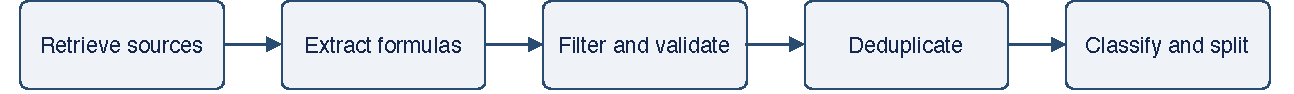
\includegraphics[width=\linewidth]{assets/dataset-pipeline.drawio.pdf}\end{center}
\end{frame}

\major{Dataset}
\begin{frame}[t]{Dataset}
\relax
\begin{center}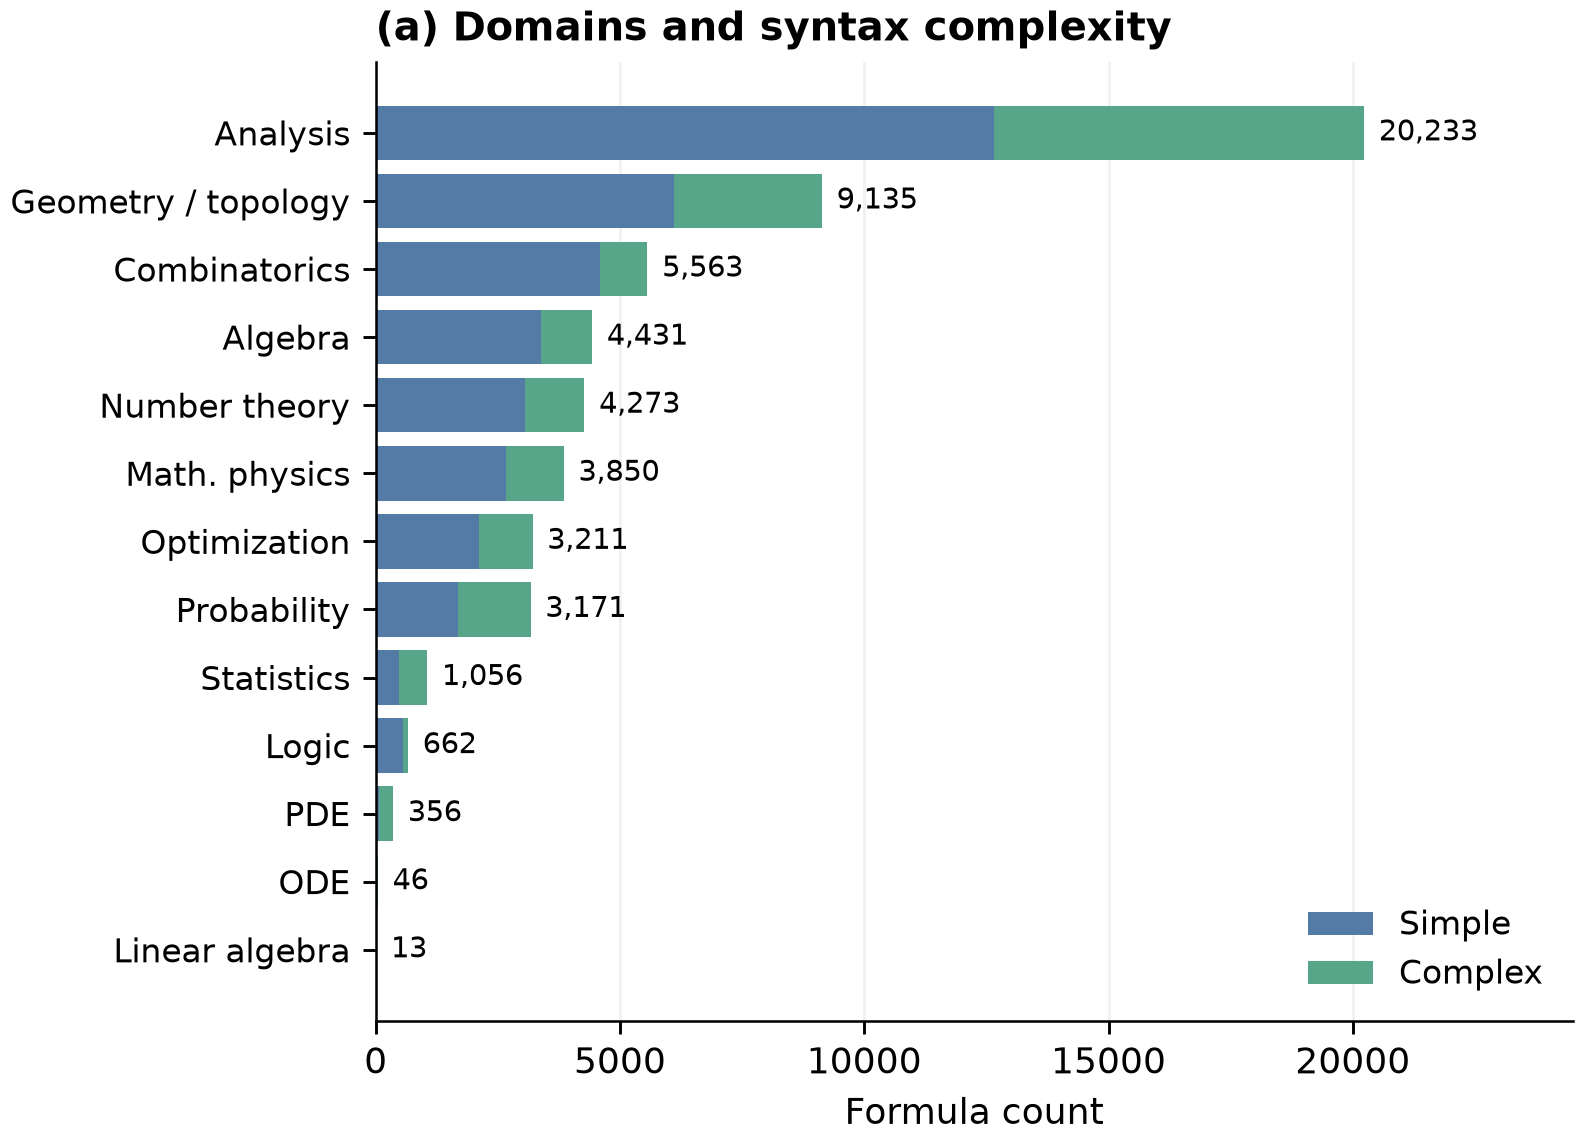
\includegraphics[width=.96\linewidth,height=7.4cm,keepaspectratio]{assets/dataset_domains_only.png}\end{center}
\end{frame}

\major{Dataset}
\begin{frame}[t]{Dataset}
\relax
\begin{columns}[T,onlytextwidth]\begin{column}{.61\linewidth}\textbf{Formula types}\par\par\noindent{\scriptsize\tbl\begin{tabularx}{\linewidth}{@{}>{\raggedright\arraybackslash}X r >{\raggedright\arraybackslash}X r@{}}\toprule
Formula type & Count & Formula type & Count\\\midrule
analysis & 20,233 & geometry / topology & 9,135\\
combinatorics & 5,563 & algebra & 4,431\\
number / theory & 4,273 & mathematical / physics & 3,850\\
optimization & 3,211 & probability & 3,171\\
statistics & 1,056 & logic & 662\\
pde & 356 & ode & 46\\
linear / algebra & 13 &  & \\
\bottomrule\end{tabularx}}\par\vspace{2pt}
\end{column}\begin{column}{.36\linewidth}\textbf{Provenance labels}\par\par\noindent{\scriptsize\tbl\begin{tabularx}{\linewidth}{@{}>{\raggedright\arraybackslash}X r@{}}\toprule
Provenance label & Formulas\\\midrule
Historical human & 51,229\\
Possible mixed & 2,810\\
Unknown & 1,961\\
Fully AI generated & 0\\
\bottomrule\end{tabularx}}\par\vspace{2pt}
\vspace{4pt}\textbf{Complexity classes}\par\par\noindent{\scriptsize\tbl\begin{tabular*}{\linewidth}{@{\extracolsep{\fill}}rr@{}}\toprule
Simple & Complex\\\midrule
37,400 & 18,600\\
\bottomrule\end{tabular*}}\par\vspace{2pt}
\end{column}\end{columns}\vspace{4pt}\textbf{Complexity score}\par\[s=.40\bar L+.20\bar C+.15\bar D+.15\bar S+.10\bar O,\quad \bar z=\min(z/z_0,2).\]{\scriptsize $L$: lexemes; $C$: command types; $D$: nesting; $S$: symbol types; $O$: operators.\\Normalizers $(L_0,C_0,D_0,S_0,O_0)=(60,6,3,18,12)$; complex iff $s\ge.65$.}\par\vspace{3pt}\textbf{Example:} $\frac{1}{s^a}$ has $(L,C,D,S,O)=(9,1,1,5,2)$, hence $s\approx0.202<0.65$: simple.\par\vspace{5pt}\textbf{Train: 36,615 formulas; validation: 7,693; test: 11,692.}
\note{The example matches the stored complexity metadata for the accepted formula. Train=v6_train, validation=v6_dev, test=union of v6_fresh_test,v7_external_test,v8_external_test. These are disjoint and sum to56000. The scenario-specific fitting scopes remain described in the retained experimental settings.}

\end{frame}

\major{Math-Atom BPE}
\begin{frame}[t]{Route 1: Learning a Mathematical Lexical Alphabet}
\relax
\begin{definitionbox}{Training alphabet}
\[A=\{\text{all 256 bytes}\}\cup\operatorname{Top}_{384}\{\text{observed complete commands / Unicode units}\}.\]Atoms are derived from fit records only, ranked by frequency with deterministic tie rules. The actual primitive counts are 596 (broad) and 495 (specialized).
\end{definitionbox}
\par\noindent{\scriptsize\tbl\begin{tabularx}{\linewidth}{@{}L{2.3cm}>{\raggedright\arraybackslash}X >{\raggedright\arraybackslash}X@{}}\toprule
Stage & Implementation & Budget accounting\\\midrule
Reversible codec & Map observed lexical units to private-use symbols. & One primitive ID per atom; unknown strings retain byte coverage.\\
Vocabulary training & Original HF BPE on fit + the allowed 512-record auxiliary pool. & Total IDs capped at 1,024 or 2,048.\\
Inference & Native lexical codec, then original Rust BPE. & No AST path search and no policy network.\\
\bottomrule\end{tabularx}}\par\vspace{2pt}
\begin{remarkbox}{Why this route remains}
It is the simple, fast mathematical reference against which extra structural machinery must justify itself. No manually enumerated command vocabulary is required.
\hyperlink{ref-bpe}{(1)} \hyperlink{ref-cmer}{(7)}
\end{remarkbox}

\end{frame}

\major{Math-Atom BPE}
\begin{frame}[t]{Route 1: Exact Source Fidelity and Its Limits}
\relax
\begin{definitionbox}{Raw-string contract}
For every evaluated $x$, $\operatorname{decode}(\operatorname{encode}(x))=x$. The ordered token byte payloads also concatenate to $\operatorname{UTF8}(x)$ exactly. No whitespace normalization is permitted.
\end{definitionbox}
\par\noindent{\scriptsize\tbl\begin{tabularx}{\linewidth}{@{}L{2.4cm}>{\raggedright\arraybackslash}X >{\raggedright\arraybackslash}X@{}}\toprule
Case & Behavior & What is not guaranteed\\\midrule
Seen command / Unicode atom & Codec retains the complete observed unit. & A larger token can still span an argument boundary.\\
Unseen command & Explicit byte coverage; no unknown-token deletion. & Every novel command need not be a single token.\\
Spacing / multiline source & Bytes are preserved exactly. & Layout variants need not receive identical token sequences.\\
Numbers / identifiers & BPE learns recurrent sequences. & Numeric magnitude is not encoded continuously.\\
\bottomrule\end{tabularx}}\par\vspace{2pt}
\begin{remarkbox}{Interpretation}
High command integrity reflects observed alphabet coverage, not universal LaTeX grammar coverage or a learned theorem representation.
\hyperlink{ref-xval}{(10)} \hyperlink{ref-texbleu}{(11)}
\end{remarkbox}

\end{frame}

\major{Boundary AST}
\begin{frame}[t]{Route 2: Source Structure as a Segmentation Cost}
\relax
\begin{definitionbox}{Same vocabulary, different path}
An edge $(a,b)$ matches $x_{a:b}\in V$ at permitted lexical endpoints. The restricted parser supplies source spans and matched brace-content endpoints.
\end{definitionbox}
\begin{definitionbox}{Additive objective}
\[z^*=\arg\min_{z\in\mathcal P(x,V)}\left[|z|+\lambda\sum_{e\in z}c_T(e)+\mu\sum_{e\in z}c_B(e)\right].\]$c_T$: token partially crosses a native source span.\\$c_B$: number of brace-content endpoints strictly inside the token.\\Development selection: $\lambda=.25$, $\mu=.30$.
\end{definitionbox}
\begin{remarkbox}{A source-tree method}
The parser is restricted and falls back to source syntax. It is not a full TeX interpreter or a semantic operator tree for arbitrary mathematics.
\hyperlink{ref-pathpiece}{(8)} \hyperlink{ref-mathgpt}{(9)}
\end{remarkbox}

\end{frame}

\major{Boundary AST}
\begin{frame}[t]{Route 2: Exact Dynamic Programming on a Fixed Graph}
\relax
\begin{definitionbox}{Backward recurrence}
\[D[n]=0,\qquad D[a]=\min_{(a,b)\in E}\{1+\lambda c_T(a,b)+\mu c_B(a,b)+D[b]\}.\]A byte trie enumerates matching dictionary edges. A stored best endpoint reconstructs the token sequence. This is exact for the specified legal graph and additive objective.
\end{definitionbox}
\par\noindent{\scriptsize\tbl\begin{tabularx}{\linewidth}{@{}L{2.0cm}>{\raggedright\arraybackslash}X >{\raggedright\arraybackslash}X@{}}\toprule
Design & Mechanism & Reason\\\midrule
Lexical mask & Suppress cuts inside covered commands / codepoints. & Keep complete observed primitive units.\\
Tree cost & Endpoint sweeps detect partial span crossings. & Avoid testing every token against every span.\\
Boundary cost & Prefix sums count hidden brace-content endpoints. & Recover argument boundaries without hard blocking all compression.\\
\bottomrule\end{tabularx}}\par\vspace{2pt}
\begin{remarkbox}{Scope of optimality}
The result is not globally optimal vocabulary learning, and a low source-tree cost does not imply low task loss. The shortest-path algorithm itself is established.
\hyperlink{ref-pathpiece}{(8)} \hyperlink{ref-greed}{(12)}
\end{remarkbox}

\end{frame}

\major{Boundary AST}
\begin{frame}[t]{Route 2: Development Selection and Runtime Cost}
\relax
\par\noindent{\scriptsize\tbl\begin{tabularx}{\linewidth}{@{}L{3.0cm}>{\raggedright\arraybackslash}X@{}}\toprule
Setting & Values / behavior\\\midrule
Prespecified grid & $\lambda\in\{0,.25,.75\}$; $\mu\in\{0,.05,.15,.30\}$: 12 candidates.\\
Selection criterion & Common old-dev utility plus .04 times missing parameter-boundary recall.\\
Feasibility guard & Compression regression at most 1\%; boundary recall loss at most 1 percentage point vs. math-atom BPE.\\
Selected setting & All four budget/scenario conditions selected .25 / .30 before v8 scoring.\\
Public encoder & C frontend + trie + DP; all source parsing is included in throughput.\\
\bottomrule\end{tabularx}}\par\vspace{2pt}
\begin{remarkbox}{Engineering and trade-offs}
Typical lattice work scales with input bytes, maximum piece length and source spans; the dense byte trie uses more memory than a compact sparse trie.\\Compared with the older length-first path, the boundary term costs some speed but restores much of the parameter-boundary recall.
\end{remarkbox}
\begin{definitionbox}{Deployment contract}
A frozen dictionary and weights define deterministic IDs. Unknown lexical units use byte coverage; supported source parsing has an explicit one-million-byte input limit.
\end{definitionbox}

\end{frame}

\major{Experimental Design}
\begin{frame}[t]{Common Inputs, Training Information and Timing}
\relax
\par\noindent{\footnotesize\tbl\begin{tabularx}{\linewidth}{@{}L{3.0cm}>{\raggedright\arraybackslash}X@{}}\toprule
Axis & Controlled implementation\\\midrule
Vocabulary budgets & 1,024 / 2,048 for trained methods; all primitive and reserved IDs count.\\
Allowed data & Identical scenario fit/auxiliary pools; generic trainers receive their union.\\
Test input & Original accepted raw strings; no per-model filtering, truncation or normalization.\\
Probability calibration & Same fit IDs for each scenario; mature models recalibrated for broad and specialized separately.\\
Timing & Seven shuffled/interleaved full public encode/decode runs; median throughput; caches cleared.\\
Statistical unit & Paper groups, not individual formulas copied across seeds.\\
\bottomrule\end{tabularx}}\par\vspace{2pt}
\begin{remarkbox}{Remaining asymmetry}
Historical tuning counts and training wall time differ. Mature vocabulary budgets differ. These differences are disclosed rather than described as fully equal compute.
\end{remarkbox}

\end{frame}

\major{Evaluation Metrics}
\begin{frame}[t]{Efficiency, Fidelity and Information Measures}
\relax
\par\noindent{\scriptsize\renewcommand{\tbl}{\renewcommand{\arraystretch}{1.27}\setlength{\tabcolsep}{3pt}}\tbl\begin{tabularx}{\linewidth}{@{}L{3.3cm}>{\raggedright\arraybackslash}X@{}}\toprule
Metric & Definition / interpretation\\\midrule
Paper-macro tokens/byte $\downarrow$ & $\frac1P\sum_p T_p/B_p$; prevents long papers from dominating the primary compression average.\\
Length distribution & Tokens/formula and 50th/95th/99th percentiles; inspect long-tail inflation.\\
Exact fidelity & Both decoded strings and concatenated raw token payloads equal the source.\\
Encode / decode speed & Raw UTF-8 MiB/s through the complete public interface.\\
Fit unigram BPB $\downarrow$ & $-B^{-1}\sum_i\log_2[(c_i+\alpha)/(N+\alpha|V|)]$; fit-only count model, not LM perplexity.\\
Information / utilization & Renyi efficiency at $\alpha=1,2,2.5,3$; used IDs / actual vocabulary.\\
\bottomrule\end{tabularx}}\par\vspace{2pt}
\begin{remarkbox}{Sensitivity}
Report smoothing at .01 / .1 / .5 / 1. Information efficiency and token count measure different properties; neither alone proves downstream quality.
\hyperlink{ref-greed}{(12)} \hyperlink{ref-tokeval}{(13)}
\end{remarkbox}

\end{frame}

\major{Evaluation Metrics}
\begin{frame}[t]{Structure, Integrity and Robustness}
\relax
\par\noindent{\scriptsize\tbl\begin{tabularx}{\linewidth}{@{}L{3.0cm}>{\raggedright\arraybackslash}X >{\raggedright\arraybackslash}X@{}}\toprule
Metric & Definition & Evidence boundary\\\midrule
Command / number integrity & Fraction of reference lexemes with no internal token cut. & Does not require isolation as a standalone token.\\
Lexical boundary P/R/F1 & Token endpoints against reference lexical endpoints. & A byte tokenizer can obtain high recall.\\
KaTeX crossing rate & Tokens partially overlapping a reference syntax span / all tokens. & A whole-formula token can obtain low crossing.\\
Parameter-boundary recall & pylatexenc group-content endpoints retained as token boundaries. & Independent implementation; syntax proxy, not semantic gold.\\
Robustness & Layout token variation; local symbol edit effects outside a 16-byte neighborhood. & The local edit is not mathematical equivalence.\\
\bottomrule\end{tabularx}}\par\vspace{2pt}
\begin{remarkbox}{Coverage is part of the result}
Unicode integrity, parser coverage and probe counts accompany the scores. No formula disappears from the common test merely because a diagnostic parser cannot measure it.
\hyperlink{ref-tokeval}{(13)} \hyperlink{ref-texbleu}{(11)}
\end{remarkbox}

\end{frame}

\major{Experimental Audit}
\begin{frame}[t]{Three New Review Rounds of the Retained Release}
\relax
\par\noindent{\scriptsize\tbl\begin{tabularx}{\linewidth}{@{}L{2.5cm}>{\raggedright\arraybackslash}X L{2.8cm}@{}}\toprule
Round & Checks actually executed & Scope\\\midrule
1. Data / provenance & Reclassify every formula; verify file IDs, hash, license/origin rules and source-disjoint pools. & 56,000 catalog records.\\
2. Public-encoder replay & Reload every current model; reconstruct original payload; replay length, reference crossings and parameter boundaries. & 234,556 formula-result rows.\\
3. Independent aggregation & Recompute paper averages, integrity and fit-calibrated probability bits; check common dictionary and seven timing repeats. & 19 configurations, 109 metric records.\\
\bottomrule\end{tabularx}}\par\vspace{2pt}
\begin{definitionbox}{Status}
All three new reviews passed. The earlier v8 freeze/evaluation additionally passed eight protocol/result checks and 201 implementation tests.
\end{definitionbox}
\begin{remarkbox}{Reorganization integrity}
Selected checkpoints are byte-identical copies of the frozen v8 artifacts. Current results are the seven-method subset, with no new training or test-based parameter changes.
\end{remarkbox}

\end{frame}

\major{Results}
\begin{frame}[t]{New-Paper Results: 1,024-ID Trained Vocabulary}
\relax
Common test: 4,294 formulas from 27 new source papers.\par\vspace{2pt}\par\noindent{\scriptsize\tbl\begin{tabular*}{\linewidth}{@{\extracolsep{\fill}}L{3.0cm}rrrrrr@{}}\toprule
System & T/B $\downarrow$ & Cross\% $\downarrow$ & Scope\% $\uparrow$ & Cmd\% $\uparrow$ & Num\% $\uparrow$ & MiB/s $\uparrow$\\\midrule
\textbf{Boundary AST (ours)} & 0.3900 & 18.43 & 64.36 & 99.76 & 97.41 & 29.68\\
\textbf{Math-atom BPE (ours)} & 0.3943 & 19.26 & 62.83 & 99.76 & 97.41 & 10.20\\
Byte BPE & 0.4121 & 25.51 & 67.62 & 62.28 & 97.43 & 8.59\\
SP Unigram & 0.4912 & 22.34 & 68.64 & 2.49 & 98.08 & 23.42\\
Qwen2.5 & 0.5318 & 21.62 & 84.76 & 2.16 & 97.41 & 3.14\\
Llama 3 & 0.5279 & 21.74 & 84.76 & 2.16 & 99.28 & 8.94\\
o200k & 0.5246 & 22.24 & 84.91 & 2.19 & 99.28 & 14.32\\
\bottomrule\end{tabular*}}\par\vspace{2pt}
\begin{definitionbox}{Reading the table}
T/B is paper-macro tokens per UTF-8 byte. Crossing and scope recall use different external syntax references; improving one does not imply improving the other.
\end{definitionbox}
\begin{remarkbox}{Comparison scope}
The two proposed systems share a dictionary. Byte BPE and Unigram share the ID budget and allowed data. Qwen2.5, Llama 3 and o200k retain their full vocabularies.
\end{remarkbox}

\end{frame}

\major{Results}
\begin{frame}[t]{New-Paper Results: 2,048-ID Trained Vocabulary}
\relax
Common test: 4,294 formulas from 27 new source papers.\par\vspace{2pt}\par\noindent{\scriptsize\tbl\begin{tabular*}{\linewidth}{@{\extracolsep{\fill}}L{3.0cm}rrrrrr@{}}\toprule
System & T/B $\downarrow$ & Cross\% $\downarrow$ & Scope\% $\uparrow$ & Cmd\% $\uparrow$ & Num\% $\uparrow$ & MiB/s $\uparrow$\\\midrule
\textbf{Boundary AST (ours)} & 0.3296 & 24.17 & 53.87 & 99.76 & 97.89 & 28.65\\
\textbf{Math-atom BPE (ours)} & 0.3372 & 24.87 & 51.18 & 99.76 & 97.57 & 9.56\\
Byte BPE & 0.3504 & 31.46 & 59.79 & 74.75 & 97.61 & 8.81\\
SP Unigram & 0.4625 & 24.03 & 67.07 & 4.16 & 98.71 & 23.54\\
Qwen2.5 & 0.5318 & 21.62 & 84.76 & 2.16 & 97.41 & 3.14\\
Llama 3 & 0.5279 & 21.74 & 84.76 & 2.16 & 99.28 & 8.94\\
o200k & 0.5246 & 22.24 & 84.91 & 2.19 & 99.28 & 14.32\\
\bottomrule\end{tabular*}}\par\vspace{2pt}
\begin{definitionbox}{Reading the table}
T/B is paper-macro tokens per UTF-8 byte. Crossing and scope recall use different external syntax references; improving one does not imply improving the other.
\end{definitionbox}
\begin{remarkbox}{Comparison scope}
The two proposed systems share a dictionary. Byte BPE and Unigram share the ID budget and allowed data. Qwen2.5, Llama 3 and o200k retain their full vocabularies.
\end{remarkbox}

\end{frame}

\major{Results}
\begin{frame}[t]{Strict Source-Domain Generalization}
\relax
Common holdout: 1,428 formulas. Specialized training excludes target and adjacent source categories.\par\vspace{2pt}\par\noindent{\scriptsize\tbl\begin{tabular*}{\linewidth}{@{\extracolsep{\fill}}L{3.5cm}rrrr@{}}\toprule
System & T/B: 1,024 & T/B: 2,048 & Scope\%: 1,024 & Scope\%: 2,048\\\midrule
Boundary AST (ours) & 0.4372 & 0.4010 & 61.27 & 53.43\\
Math-atom BPE (ours) & 0.4470 & 0.4118 & 60.70 & 53.72\\
Byte BPE & 0.4726 & 0.4188 & 66.29 & 61.13\\
SP Unigram & 0.5325 & 0.5011 & 70.89 & 70.10\\
Qwen2.5 & 0.5415 & 0.5415 & 86.87 & 86.87\\
Llama 3 & 0.5353 & 0.5353 & 86.87 & 86.87\\
o200k & 0.5335 & 0.5335 & 86.63 & 86.63\\
\bottomrule\end{tabular*}}\par\vspace{2pt}
\begin{definitionbox}{What generalizes}
Boundary AST compresses more than the same-dictionary BPE in both budgets. Scope recall changes by +0.57 pp / -0.28 pp; not every structural diagnostic improves.
\end{definitionbox}
\begin{remarkbox}{What remains uncertain}
Source categories are disjoint by construction, but mathematical concepts can overlap. Few source papers and uneven domains produce wide uncertainty intervals.
\end{remarkbox}

\end{frame}

\major{Results}
\begin{frame}[t]{Compression Across Vocabulary Budgets}
\relax
\begin{center}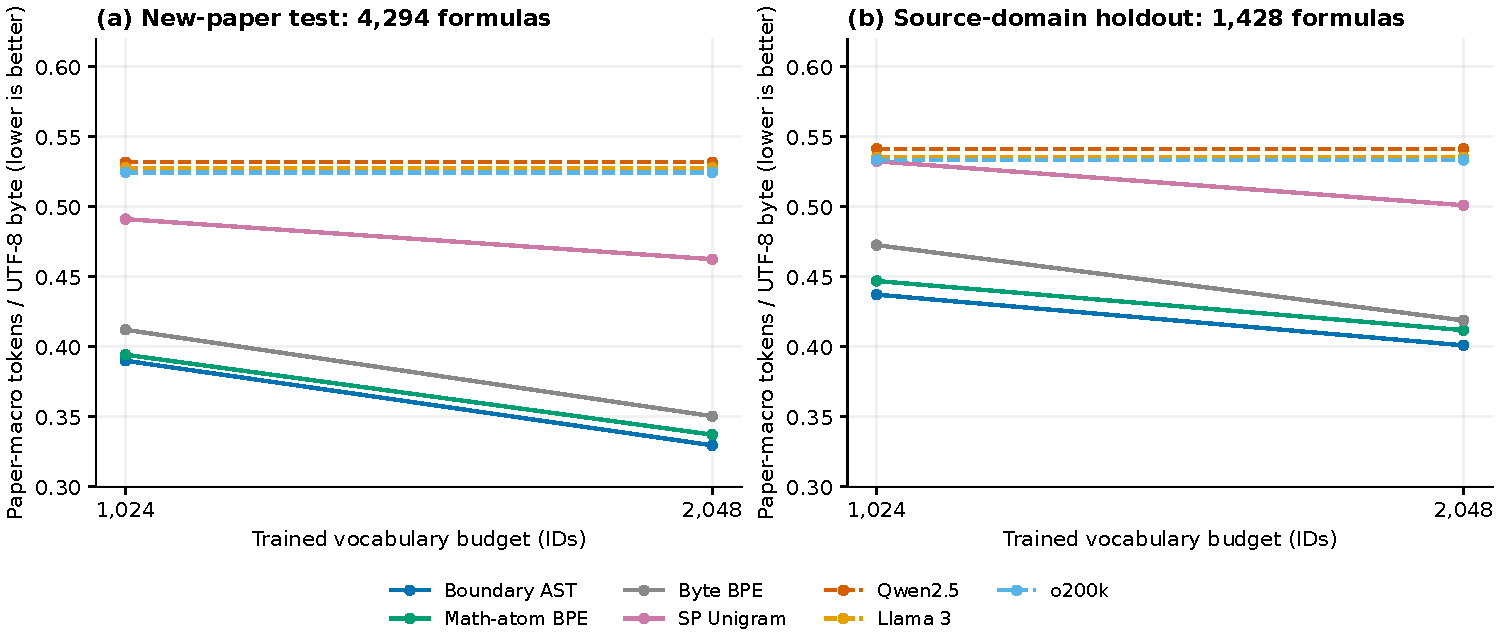
\includegraphics[width=.98\linewidth,height=5.2cm,keepaspectratio]{assets/compression_by_budget.pdf}\end{center}\begin{remarkbox}{Interpretation}
Solid lines: trained 1,024/2,048-ID systems. Dashed lines: fixed full-vocabulary general tokenizers. Lower is shorter; this is not a downstream-accuracy curve.
\end{remarkbox}

\end{frame}

\major{Results}
\begin{frame}[t]{Runtime and Source-Tree Crossing}
\relax
\begin{center}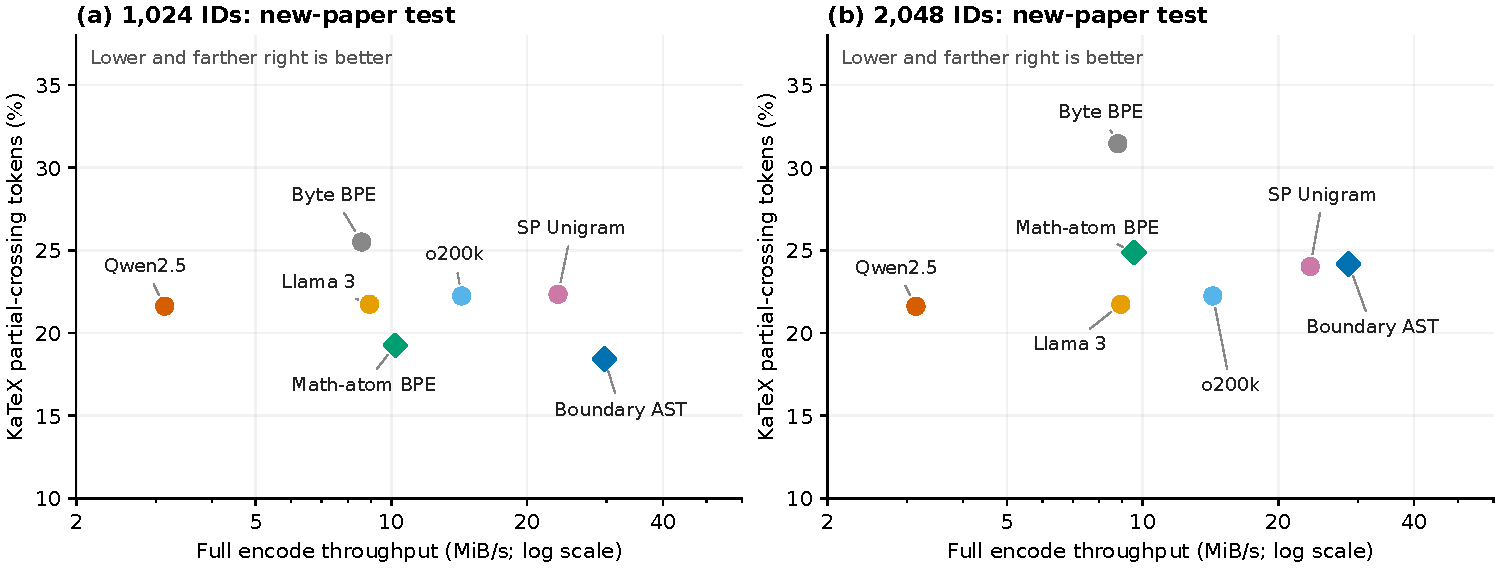
\includegraphics[width=.98\linewidth,height=5.3cm,keepaspectratio]{assets/speed_structure.pdf}\end{center}\begin{remarkbox}{Interpretation}
Boundary AST is about 2.65--3.00 times faster than math-atom BPE across the four principal conditions. All parser/codec work is included. The result is from one Mac and a single-input public interface.
\end{remarkbox}

\end{frame}

\major{Results}
\begin{frame}[t]{Paired Paper-Cluster Statistical Evidence}
\relax
Difference: Boundary AST minus math-atom BPE. Negative compression differences favor AST.\par\vspace{2pt}\par\noindent{\scriptsize\tbl\begin{tabularx}{\linewidth}{@{}L{2.4cm}r L{3.5cm}>{\raggedright\arraybackslash}X@{}}\toprule
Condition & T/B difference & Family 95\% CI & Scope difference CI (pp)\\\midrule
1,024 / broad & -0.00428 & [-0.00601, -0.00270] & [-2.36, +6.06]\\
1,024 / domain & -0.00976 & [-0.02916, -0.00197] & [-4.44, +9.88]\\
2,048 / broad & -0.00760 & [-0.01106, -0.00535] & [+0.49, +6.59]\\
2,048 / domain & -0.01088 & [-0.03025, -0.00344] & [-5.78, +12.17]\\
\bottomrule\end{tabularx}}\par\vspace{2pt}
\begin{definitionbox}{Design}
200,000 paper-cluster resamples; Bonferroni intervals retain the original family of 144 comparisons. We did not shrink the family after choosing seven systems.
\end{definitionbox}
\begin{itemize}
\item All four adjusted compression intervals exclude zero in favor of Boundary AST.
\item Scope and crossing intervals do not all exclude zero; point estimates are not universal structural gains.
\item Intervals condition on the realized vocabulary and observed training seeds. They do not cover all possible retraining outcomes.
\end{itemize}

\end{frame}

\major{Results}
\begin{frame}[t]{Probability Coding and Vocabulary Utilization}
\relax
\par\noindent{\scriptsize\tbl\begin{tabular*}{\linewidth}{@{\extracolsep{\fill}}L{3.4cm}rrrr@{}}\toprule
System & Fit BPB: 1,024 & Fit BPB: 2,048 & Used\%: 1,024 & Used\%: 2,048\\\midrule
Boundary AST (ours) & 3.131 & 3.008 & 67.3 & 72.0\\
Math-atom BPE (ours) & 3.153 & 3.028 & 66.8 & 70.9\\
Byte BPE & 3.413 & 3.209 & 76.3 & 76.3\\
SP Unigram & 3.709 & 3.634 & 69.5 & 67.2\\
Qwen2.5 & 4.063 & 4.063 & 0.8 & 0.8\\
Llama 3 & 4.056 & 4.056 & 1.1 & 1.1\\
o200k & 4.060 & 4.060 & 0.7 & 0.7\\
\bottomrule\end{tabular*}}\par\vspace{2pt}
\begin{definitionbox}{Interpretation}
Fit BPB uses the same scenario fit records and actual vocabulary size. The much larger general vocabularies incur a different smoothing term and utilization denominator.
\end{definitionbox}
\begin{remarkbox}{Why several measures are necessary}
Low token count can coexist with sparse usage or unstable boundaries. These probability readouts are descriptive token statistics; no trained language-model perplexity is reported.
\hyperlink{ref-greed}{(12)} \hyperlink{ref-tokeval}{(13)}
\end{remarkbox}

\end{frame}

\major{Results}
\begin{frame}[t]{Current Seven-System Composite Ranking}
\relax
\par\noindent{\scriptsize\tbl\begin{tabular*}{\linewidth}{@{\extracolsep{\fill}}L{3.4cm}rrrr@{}}\toprule
System & Rank: 1,024 & Rank: 2,048 & Score: 1,024 & Score: 2,048\\\midrule
Boundary AST (ours) & 1 & 1 & 0.042 & 0.100\\
Math-atom BPE (ours) & 2 & 2 & 0.271 & 0.342\\
Byte BPE & 5 & 5 & 0.610 & 0.608\\
SP Unigram & 3 & 3 & 0.433 & 0.450\\
Qwen2.5 & 7 & 7 & 0.860 & 0.817\\
Llama 3 & 6 & 6 & 0.696 & 0.646\\
o200k & 4 & 4 & 0.587 & 0.537\\
\bottomrule\end{tabular*}}\par\vspace{2pt}
\begin{definitionbox}{Frozen metric preferences}
Compression 30\%; encode speed 25\%; KaTeX crossing 20\%; command integrity 10\%; number integrity 5\%; fit BPB 10\%. Broad and specialized scenarios each receive 50\%.
\end{definitionbox}
\begin{remarkbox}{How to use the ranking}
The ranking favors our complete specialized systems under this preference. It is relative to the seven retained methods, omits scope recall from its weighted score and cannot establish downstream superiority.
\end{remarkbox}

\end{frame}

\major{Next Work}
\begin{frame}[t]{Limitations and Next Steps}
\relax
\begin{definitionbox}{Downstream tasks}
Validate the tokenizers on PDE solving, ODE solving, and mathematical reasoning beyond equation solving.
\end{definitionbox}
\par\noindent{\footnotesize\renewcommand{\tbl}{\renewcommand{\arraystretch}{1.25}\setlength{\tabcolsep}{3pt}}\tbl\begin{tabularx}{\linewidth}{@{}L{2.3cm}>{\raggedright\arraybackslash}X@{}}\toprule
Step & Experimental procedure\\\midrule
1. Architecture & Select a suitable model architecture.\\
2. Tokenizer integration & Connect each tokenizer to the same architecture.\\
3. Training & Train each model fully from scratch.\\
4. Evaluation & Select suitable benchmarks and evaluate downstream task performance.\\
\bottomrule\end{tabularx}}\par\vspace{2pt}
\begin{remarkbox}{Open issues}
\textbf{Benchmarks:} identify suitable benchmarks for each mathematical task.\\\textbf{Compute:} full training from scratch requires substantial computational resources.
\end{remarkbox}

\end{frame}

\major{References}
\begin{frame}[t]{References (1/2)}
\relax
{\scriptsize \par\noindent\hypertarget{ref-bpe}{}\textbf{(1)} Sennrich, Haddow and Birch (2016). \href{https://aclanthology.org/P16-1162/}{Neural Machine Translation of Rare Words with Subword Units}. ACL.\par\vspace{14pt}
\par\noindent\hypertarget{ref-sentencepiece}{}\textbf{(2)} Kudo and Richardson (2018). \href{https://aclanthology.org/D18-2012/}{SentencePiece: A Simple and Language Independent Subword Tokenizer and Detokenizer for Neural Text Processing}. EMNLP Demonstrations.\par\vspace{14pt}
\par\noindent\hypertarget{ref-qwen}{}\textbf{(3)} Qwen Team (2024). \href{https://arxiv.org/abs/2412.15115}{Qwen2.5 Technical Report}. Technical report.\par\vspace{14pt}
\par\noindent\hypertarget{ref-llama}{}\textbf{(4)} Dubey et al. (2024). \href{https://arxiv.org/abs/2407.21783}{The Llama 3 Herd of Models}. Technical report.\par\vspace{14pt}
\par\noindent\hypertarget{ref-tiktoken}{}\textbf{(5)} OpenAI (2026). \href{https://github.com/openai/tiktoken}{tiktoken: BPE Tokenizer Library}. Official software; accessed 2026-10-13.\par\vspace{14pt}
\par\noindent\hypertarget{ref-unigram}{}\textbf{(6)} Kudo (2018). \href{https://aclanthology.org/P18-1007/}{Subword Regularization: Improving Neural Network Translation Models with Multiple Subword Candidates}. ACL.\par\vspace{14pt}
\par\noindent\hypertarget{ref-cmer}{}\textbf{(7)} Bai et al. (2026). \href{https://ojs.aaai.org/index.php/AAAI/article/view/37224}{Complex Mathematical Expression Recognition: Benchmark, Large-Scale Dataset and Strong Baseline}. AAAI.\par\vspace{14pt}}
\end{frame}

\major{References}
\begin{frame}[t]{References (2/2)}
\relax
{\scriptsize \par\noindent\hypertarget{ref-pathpiece}{}\textbf{(8)} Schmidt et al. (2024). \href{https://aclanthology.org/2024.emnlp-main.40/}{Tokenization Is More Than Compression}. EMNLP.\par\vspace{14pt}
\par\noindent\hypertarget{ref-mathgpt}{}\textbf{(9)} Scarlatos and Lan (2023). \href{https://aclanthology.org/2023.acl-long.205/}{Tree-Based Representation and Generation of Natural and Mathematical Language}. ACL.\par\vspace{14pt}
\par\noindent\hypertarget{ref-xval}{}\textbf{(10)} Golkar et al. (2023). \href{https://arxiv.org/abs/2310.02989}{xVal: A Continuous Numerical Tokenization for Scientific Language Models}. Preprint.\par\vspace{14pt}
\par\noindent\hypertarget{ref-texbleu}{}\textbf{(11)} Jung et al. (2024). \href{https://arxiv.org/abs/2409.06639}{TeXBLEU: Automatic Metric for Evaluate LaTeX Format}. Preprint.\par\vspace{14pt}
\par\noindent\hypertarget{ref-greed}{}\textbf{(12)} Uzan et al. (2024). \href{https://aclanthology.org/2024.acl-short.73/}{Greed Is All You Need: An Evaluation of Tokenizer Inference Methods}. ACL.\par\vspace{14pt}
\par\noindent\hypertarget{ref-tokeval}{}\textbf{(13)} Meister (2026). \href{https://arxiv.org/abs/2608.18062}{TokEval: A Tokenizer Evaluation Suite}. COLM.\par\vspace{14pt}}
\end{frame}
\end{document}
